\section{Tickets}
\label{ticket}
In the HOPR protocol, nodes that have staked funds within a payment channel can issue tickets that are used for payment to other nodes.
Tickets are used for probabilistic payments; every ticket is bound to a specific payment channel and cannot be spent elsewhere.
They are redeemable at most once and they lose their value when the channel is closed or when the commitment is reset. A commitment is a secret on-chain value that is used to verify whether a ticket is a win or not when it's revealed in order to redeem it.
\subsection{Ticket issuance}
A ticket can be issued once two nodes have established a payment channel with each other which means that at least one of them has locked HOPR tokens.
\newline The ticket issuer A (A could also be the packet creator) selects the winning probability of the ticket and the relay fee to use and sets amount to:
$$\sigma=\dfrac{L\times F}{P_w}$$
where $\sigma$ is the amount of HOPR tokens set in the ticket, $L$ is the path length, $F$ is the relay fee and $P_w$ is the ticket's winning probability.
\\~\\$(A)$ issues a ticket for the next downstream node,
the challenge is given together with the routing information by the packet.
\\$(A)$ does not know whether the ticket is a win or not.
    \\$(A)$ sets the content of a ticket to: $$t=(R,\sigma,P_w,\alpha,I,T_c,\zeta)$$
\\~\\$(A)$ then signs the ticket with its private key and sends $T= (t, Sig_I(t))$ to the recipient together with a mixnet packet.
    \\~\\\textbf{Recipient's Ethereum adress $R$:} is a unique identifier that is derived from the ticket recipient's public key.
    \\\textbf{Ticket Index $I$:} is set by the ticket issuer and increases with every issued ticket. The recipient verifies that the index increases with every packet and drops packets if this is not the case. Redeeming a ticket with index $n$ invalidates all tickets with index $I<n$, hence the relayer has a strong incentive to not accept tickets with unchanged index.
    \\\textbf{Ticket challenge $T_c$:}  is set by the ticket issuer and used to check whether a ticket is redeemable before the packet is been relayed. The packet is dropped if that's not the case.
    \\\textbf{Ticket Epoch $\alpha$:} is used as a mechanism to prevent cheating by turning non-winning tickets into winning ones. This is done by increasing the value of $\alpha$ whenever a node resets a commitment which helps keeping track of updates to the on-chain commitments and invalidates tickets with the previous epoch.
    \\\textbf{Channel Epoch $\zeta$:} is used to give each reincarnation of the payment channel a new identifier such that tickets issued for previous instances of the channel lose their validity once a channel is reopened ($\alpha$'s count restarts again). This is due to the fact that $\zeta$ increments whenever a closed channel is re(-opened).
    \begin{comment}
        
   
    \\\textbf{ChainId $c_{Id}$:} The channel identifier which is defined by the ticket issuer in order to determine which channel will be used between issuer and recipient. For example, tickets that are valid on xDAI are not valid on Ethereum.
    \\\textbf{Tag $\tau$} is given as a constant and depends on the utilized blockchain. It is used to distinguish HOPR tickets from others with the same structure that are meant for different payment channels and invalidates their usage in HOPR.
    \\\textbf{Version $V$} is given as a constant and depends on the utilized blockchain. It is used to invalidate tickets that were issued for previous versions of HOPR from being used in future iterations of the protocol.

\end{comment}

    \begin{figure}[H]
        \centering
        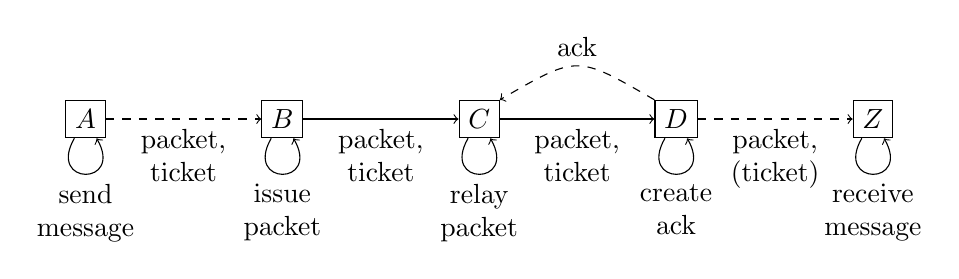
\begin{tikzpicture}[auto]
            \draw (0,0) node (a) [rectangle,draw] {$A$};
            \draw (2.5,0) node (b) [rectangle,draw] {$B$};
            \draw (5,0) node (c) [rectangle,draw] {$C$};
            \draw (7.5,0) node (d) [rectangle,draw] {$D$};
            \draw (10,0) node (z) [rectangle,draw] {$Z$};

            \draw [->,draw,dashed] (a.east) to node [align=center,below] {packet,\\ticket} (b.west);
            \draw [->,draw] (b.east) to node [align=center,below] {packet,\\ticket} (c.west);
            \draw [->,draw] (c.east) to node [align=center,below] {packet,\\ticket} (d.west);
            \draw [->,draw,dashed] (d.east) to node [align=center,below] {packet,\\(ticket)}  (z.west);

            \path[->] (a) edge [out=-120,in=-60,distance=2em,below] node [align=center] {send\\message}  (a);    % \draw 
            \path[->] (b) edge [out=-120,in=-60,distance=2em,below] node [align=center] {issue\\packet}  (b);    % \draw 
            \path[->] (c) edge [out=-120,in=-60,distance=2em,below] node [align=center] {relay\\packet}  (c);    % \draw 
            \path[->] (d) edge [out=-120,in=-60,distance=2em,below] node [align=center] {create\\ack}  (d);    % \draw 
            \path[->] (z) edge [out=-120,in=-60,distance=2em,below] node [align=center] {receive\\message}  (z);    % \draw 

            \path[->,draw,looseness=1.5,dashed,bend right] (d.north west) to [above] node {ack} (c.north east);
        \end{tikzpicture}    \caption{Ticket workflow}
        \label{fig:Ticket worklow}
    \end{figure}


\subsection{Ticket validation}
Tickets are received together with packets which means that the recipient and the next downstream node share a secret $s$ whose key shares $s_i$ and $s_{i+1}$ are derivable by those nodes.
\\~\\ \textbf{Validate response:} Once $(A)$ receives $s_{i+1}^{(1)}$ from (B) by the secret sharing, it can compute $$r_i=s_i^{(0)}+s_{i+1}^{(1)}$$ where $r_i$ is the response $r$ at iteration $i$ such that it verifies
$$r_i*G=T_{c_i}$$
\\\textbf{Validate hint:} Once the recipient transforms the packet, it is able to compute $s_i$. The recipient is now also able to extract the routing information from the packet.
This includes a hint to the value $s_{i+1}$ given as $$H_i=s_{i+1}^{(1)}*G$$ which is stored in the Sphinx packet header.
\\The unacknowledged ticket is stored in the database under the hint to the promised value to make sure that the acknowledgement can be afterwards linked to the unacknowledged ticket.
\newline Together with $s_i^{(0)}$, the node can verify that $$T_{c_i}=s_i^{(0)}*G+H_i$$ with $$s_i^{(0)}*G+H_i=s_i^{(0)}*G+s_{i+1}^{(1)}*G=(s_i^{(0)}+s_{i+1}^{(1)})*G$$
This allows the recipient to verify that the promised value $s_{i+1}^{(1)}$ indeed leads to a solution of the challenge given in the ticket.
If this is not the case, then the node should drop the packet.
\newline Without this check, the sender is able to intentionally create falsy challenges that lead to unredeemable tickets.


\subsection{Ticket redemption}


In order to unlock the ticket, the node (ticket recipient) stores it within its database until it receives an acknowledgement containing $s_{i+1}$ from the next downstream node. The challenge can be computed from acknowledgement as $T_{c_i}=ack_i*G$. The node checks the following in order to redeem tickets:
\begin{itemize}
\item Channel \textbf{exists} and is \textbf{open} or \textbf{pending to close}. The check happens locally and not on-chain using the blockchain indexer in order not to reveal any metadata. If the node does not have a record about the channel or considers the channel to be in a state different from \textbf{open} or \textbf{pending to close}, the ticket is dropped and the reception of the accompanying packet is rejected.

    \item Once it receives an acknowledgement, it checks whether it stores an unacknowledged ticket for the received acknowledgement.
If this is not the case, the node should drop the acknowledgement.
\newline The node then computes the response to the challenge (which we can also refer to as \textit{proof of relay secret}) given in the ticket as $$r_i=(s_i^{(0)}+s_{i+1}^{(1)})*G$$
\item Additionally, the node retrieves the next commitment value $comm_{i-1}$, checks that this value is not empty and that commitment is the hash of next commitment as follows:
$$ comm_{i-1} != 0 \; and \; comm_{i}=h(comm_{i-1})$$
\item The node then verifies that $r_i$ and $comm_{i-1}$ lead to a winning ticket.
This is the case if $$h(t_h, r_i, comm_{i-1} ) <P_w$$ where $t_h=h(t)$ is the ticket hash and $h$ is a hash function.
If this is not the case, the node should drop the ticket.
The final recipient of the packet does not receive a ticket because message reception is not incentivized by the HOPR protocol.
\item  The node checks whether the information gained from the packet transformation is sufficient to fulfill the given challenge sent along with the ticket. $$r_i*G=T_{c_i}$$
It then replies with an acknowledgement that includes a response to the challenge.
\item Ticket signer must be the ticket issuer. This is done using the $$ECDSA.recover()$$ ethereum function which recovers the private key used to sign $T= (t, Sig_I(t))$ and verifies if the associated public key is the issuer's public key. The packet is dropped if this test fails.
\item Ticket Epoch $\alpha$ and channel Epoch $\zeta$ must be equal to the account nonces (current values in the smart contract) $$\alpha=\alpha_c \;\; and \;\; \zeta=\zeta_c$$
where $\alpha_c$ and $\zeta_c$ represent the current values in the smart contract.
\item The ticket hasn't been already redeemed and ticket index is strictly greater than the current value in the smart contract (replay protection).
     $$I_c <I$$ where $I_c$ is the current value in the smart contract and $I$ the ticket index.
\item Channel must have enough funds to cover the costs for the ticket: $$ C_b>\sigma$$ where $\sigma$ is the ticket amount and $C_b$ is the channel balance.
   


\end{itemize}








